% Chapter 3: Methodology

This chapter describes the methods and approaches used in the experiments. This includes the selection of dataset, models, loss functions, and evaluation strategies.

\section{Overview of Approach}

Image classification involves predicting the correct category of an image from a set of predefined classes. This project focuses on addressing the challenge of class imbalance, where some classes have many samples while others have very few.

The CIFAR-100 dataset \cite{krizhevsky2009learning} was chosen because it is small enough to work with efficiently and is commonly used in other research. To create a long-tailed version of the dataset, its class distribution was adjusted to match the distribution of the ImageNet-LT dataset used in \cite{zhang2023deep}. This adjustment ensures that the experiments simulate real-world class imbalance.

Several loss functions designed to handle class imbalance were tested in this project, including Softmax Cross-Entropy (CE), Focal Loss (FL), Class-Balanced (CB) Loss, Balanced Softmax (BS) Loss, Equalization (EQ) Loss, and LDAM Loss. These loss functions modify how the models learn, making it easier for them to focus on classes with fewer samples.

The experiments were performed using four model architectures: ResNet50, MobileNetV2, ConvNeXt Base, and ViT-B/16. All models were pretrained on ImageNet, which provided a strong starting point for fine-tuning on the CIFAR-100 dataset. These models were chosen because they are well-suited for image classification tasks and represent different design approaches.

Each model was trained on both a balanced training set and a long-tailed training set. The performance of the models was evaluated using a balanced test set, a long-tailed test set, and the long-tailed test set divided into head, middle, and tail classes. This division made it possible to analyze the performance for classes with different numbers of samples. The main evaluation metric used was top-1 accuracy, which measures how often the model's top prediction is correct.

In what follows, each step of the methodology will be explained in detail.

\section{Dataset Preparation and Specifications}
A description of this section here.

Following the dataset structure used in \textit{Deep Long-Tailed Learning: A Survey}, the CIFAR100 dataset was modified to create a long-tailed training set and a balanced test set. 

\subsection{Benchmark Dataset Selection}
There are a number of benchmark datasets for long-tailed image classification tasks, including ImageNet-LT, Places365-Lt, CIFAR-100-LT, and iNaturalist 2018 \todo{references}. The previous three are sampled from ImageNet, Places365, and CIFAR-100, following the Pareto distribution, as described in section \ref{sec:lt-datasets}, while the iNaturalist 2018 is a natural long-tailed dataset. Table \ref{tab:datasets} summarizes the four datasets and their data specifications. 

\begin{table}[ht]
    \centering
    \caption{Summary of long-tailed benchmarks for image classification.}
    \begin{tabular}{lccc}
    \hline
    \textbf{Dataset}           & \textbf{\# Classes} & \textbf{\# Training Data} & \textbf{\# Test Data} \\ \hline
    ImageNet-LT   & 1,000              & 115,846                   & 50,000                \\
    CIFAR100-LT   & 100                & 50,000                    & 10,000                \\
    Places-LT     & 365                & 62,500                    & 36,500                \\
    iNaturalist 2018 & 8,142            & 437,513                   & 24,426                \\ \hline
    \end{tabular}
    \label{tab:datasets}
\end{table}
    

With its 100 classes and only 60,000 samples, the CIFAR-100 dataset was chosen as a benchmark for the experiments conducted in this thesis based on its managable size, compared to the other benchmarks, and widespread use as a standard in image classification research \todo{reference}. It's comparatively small size allows for rapid experimentation and comparisons, wheras a larger benchmark requires more computational effort and time for experiments, thus it is well-suited for multiple configurations and evaluations. However, CIFAR-100 has some limitations comparet to larger dataset, like ImageNet-LT or iNaturalist. For example, CIFAR-100 images are of relatively low resolution ($32 \times 32$ pixels) compared to ImageNet ($224 \times 224$ pixels), and may limit the ability of models to capture fine-grained details. Likewise, the smaller number of classes and samples can result in less diversity compared to datasets like iNaturalist 2018, which contains nearly nine times as many samples in the training data as CIFAR-100-LT. Despite these drawbacks, CIFAR-100-LT remains a practical choice for this thesis due to its computational efficiency. 

\todo{Describe the type of images in CIFAR-100 and include examples.}

\subsection{Data Characteristics: Class Distribution}
% \textit{A list of subjects to include in this section:}

% \begin{itemize}
%     \item Describe the ImageNet-LT dataset: number of classes, imbalance ratio, etc.
%     \item Describe the plots and what they mean for the CIFAR100-LT data preparation. 
% \end{itemize}
Understanding the class distribution in long-tailed datasets is essential for evaluating the impact of the class imbalance on model performance. This section analyzes the class distribution of the benchmark ImageNet-LT used in \cite{zhang2023deep}, which serves as a reference for creating a similar distribution across the CIFAR-100-LT training, evaluation, and test datasets.  

The ImageNet-LT dataset, introduced by Liu et al. \cite{liu2019largescalelongtailedrecognitionopen}, has been widely used in empirical studies, including \textit{Deep Long-Tailed Learning: A Survey} \cite{zhang2023deep}. The class distributions of its training, validation, and test sets are shown in Figures~\ref{fig:IN-train}, \ref{fig:IN-val}, and \ref{fig:IN-test}, respectively. The ImageNet-LT is constructed from the original ImageNet-2012 following the Pareto-distribution (Eq. \eqref{eq:pareto}) with power value $\alpha=6$ \cite{liu2019largescalelongtailedrecognitionopen}, resulting in an imbalance ratio of 256, meaning that the most frequent class has 256 times more samples than the least frequent class. As suggested in figure \ref{fig:IN-train}, the most frequent class has 1280 images, and the least frequent class 5 images \cite{liu2019largescalelongtailedrecognitionopen}. The power value of 6 is relatively large, resulting in the steep imbalance and very few samples in the tail, as seen in figure \ref{fig:IN-train}. The underrepresentation in the tail classes poses a significant challenge for models to learn from tail classes. Both the validation and test sets are balanced, as shown in figures \ref{fig:IN-val} and \ref{fig:IN-test}, respectively. There are 20 samples per class in the validation set, and 50 samples per class in the test set.


\begin{figure}[h!]
    \centering
    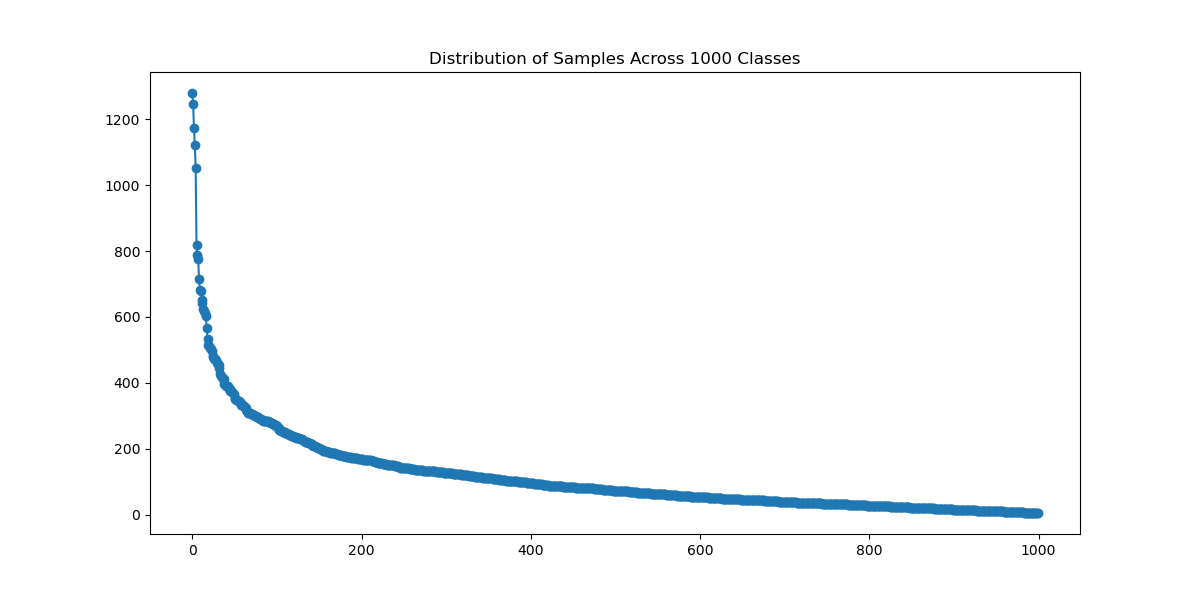
\includegraphics[width=0.9\textwidth]{Images/Plots/class_distribution_train.png}
    \caption{The class distribution of the training images for the ImageNet-LT dataset shows a long-tailed distribution.}
    \label{fig:IN-train}
\end{figure}

\begin{figure}[h!]
    \centering
    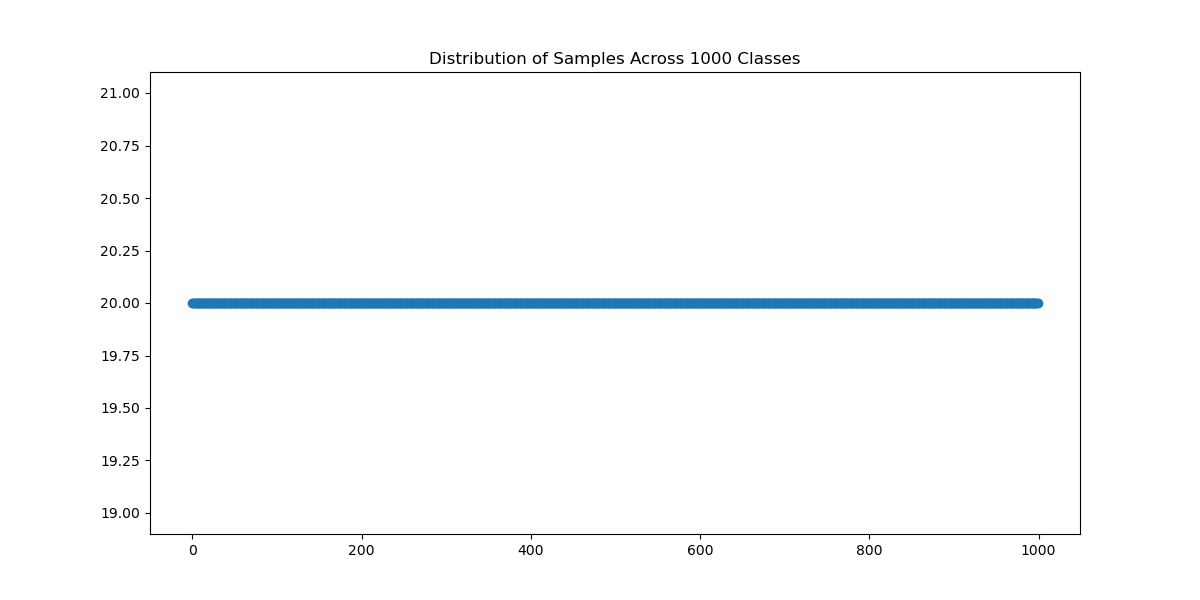
\includegraphics[width=0.9\textwidth]{Images/Plots/class_distribution_val.png}
    \caption{The class distribution of the validation images for the ImageNet-LT dataset shows that there are 20 samples of each class.}
    \label{fig:IN-val}
\end{figure}

\begin{figure}[h!]
    \centering
    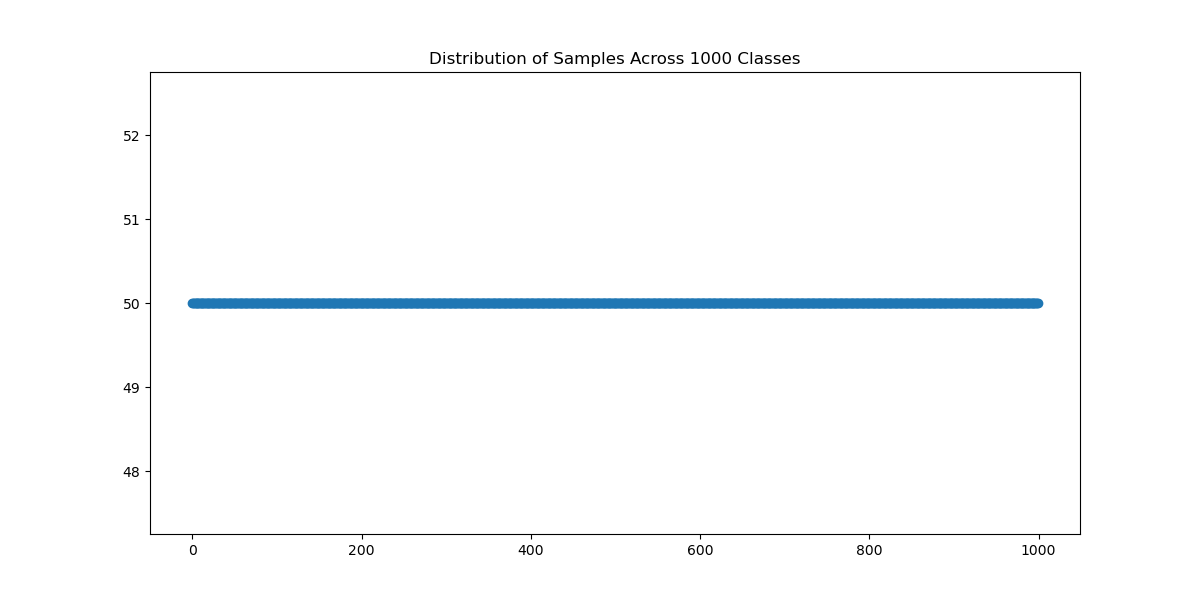
\includegraphics[width=0.9\textwidth]{Images/Plots/class_distribution_test.png}
    \caption{The class distribution of the test images for the ImageNet-LT dataset shows that there are 50 samples of each class.}
    \label{fig:IN-test}
\end{figure}


However, investigating the CIFAR-100-LT dataset used in \emph{Learning Imbalanced Datasets with Label-Distribution-Aware Margin Loss} by Cao et al. \cite{cao2019learningimbalanceddatasetslabeldistributionaware} shows that the training dataset follows a exponential decay, and not a pareto distribution. The imbalance factor in their studies is 100, meaning that the most frequent class has 100 times more samples than the least frequent class, according to equation \eqref{eq:exp}. This means that the imbalance is not as steep as with the Pareto distribution, resulting in a middle section of classes with fewer samples than the head classes, but more samples than the tail classes, see figure \ref{fig:cifar100_imbalance_cifar}. The following section will describe the preparation of CIFAR-100 for the experiments in this thesis.


\subsection{Preparation: CIFAR100-LT}
\textit{A list of subjects to include in this section:}

\begin{itemize}
    \item Explain why the dataset was saved, and not generated in run-time, like in LDAM-DRW.
    \item Explain why the dataset was split into 450 samlpes per class for training and 50 samples per class for testing.
    \item Describe the head, middle, and tail classes.
    \item Insert plot of the division of the long-tailed test dataset: head, middle, and tail classes.
\end{itemize}

The experiments conducted in this thesis are trained and evaluated on the CIFAR-100 dataset. This was downloaded using the PyTorch torchvision.datasets.CIFAR100 \cite{pytorch_cifar100}. The training and test datasets were preprocessed by converting the images to tensors using the ToTensor transformation and saved as .pth files for efficient loading during experiments. 

To address the needs of the experiments in this thesis, the original CIFAR-100 dataset was modified to create a new split of the training data. Specifically, the training data was split into 450 samples per class for training and 50 samples per class for testing, mirroring the test data for the ImageNet, maintaining the class distribution within these splits. The original test set of the CIFAR-100 dataset was retained as the validation set for evaluation during training. 

% \begin{figure}[h!]
%     \centering
%     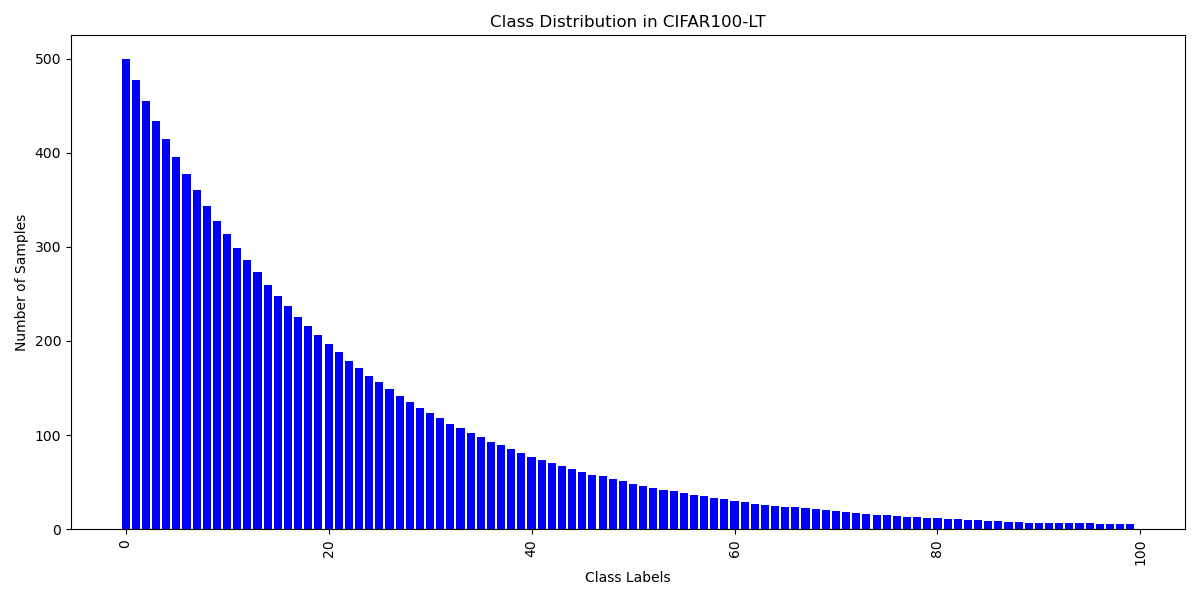
\includegraphics[width=0.9\textwidth]{Images/Plots/Class Distribution for CIFAR100-LT.png}
%     \caption{The class distribution of CIFAR100-LT with imbalance ratio 100 generated by the imbalance\_cifar.py in the LDAM-DRW GitHub repository \cite{kaidic_ldam_drw}.}
%     \label{fig:cifar100_imbalance_cifar}
% \end{figure}

% \begin{figure}[h!]
%     \centering
%     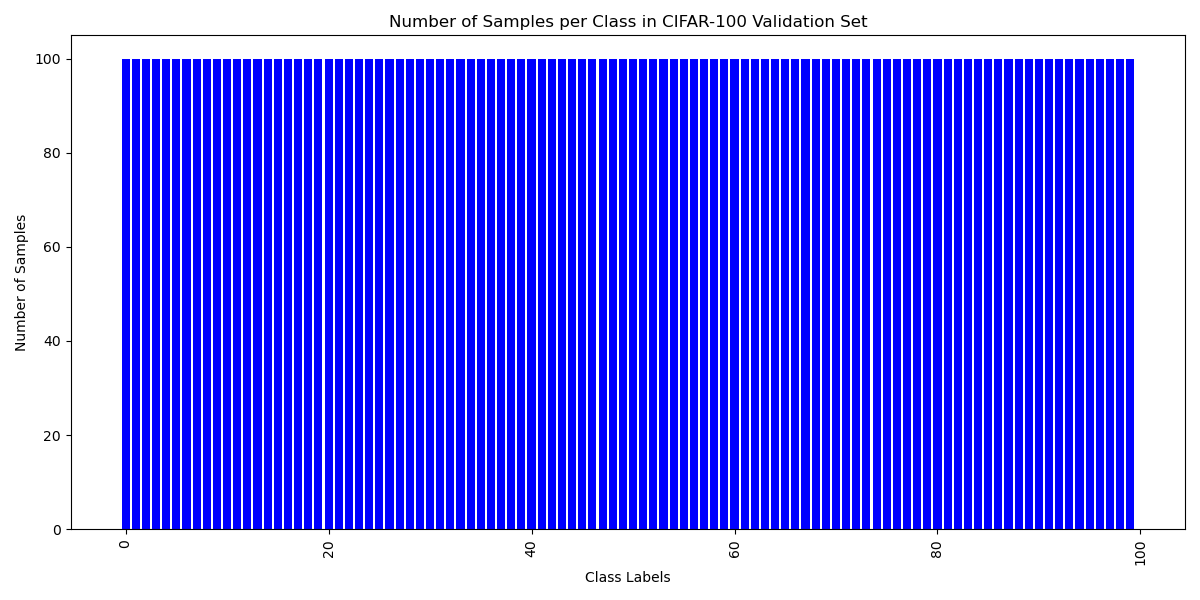
\includegraphics[width=0.9\textwidth]{Images/Plots/cifar100_val_class_distribution.png}
%     \caption{The class distribution of the CIFAR100 validation set from torchvision \cite{pytorch_cifar100}.}
%     \label{fig:cifar100val}
% \end{figure}

\textbf{Training Set:} To simulate real-world scenarios with class imbalances, the training dataset was modified to introduce an exponential imbalance across the 100 classes. The imbalance was created using exponential decay, where the number of samples per class decreases exponentially, controlled by the imbalance factor, see equation \eqref{eq:exp}. For this thesis, an imbalance factor of 0.01 was applied. This means that the most frequent class contains a 100 times more samples than the least frequent class. 

The resulting class distribution varied from the most frequent class having 450 samples to the least frequent class having only 4 samples, as shown in figure \ref{fig:cifar100_train_450_imb}. This imbalance ensured no class was left with zero samples, maintaining the integrity of all classes for training.

\begin{figure}[h!]
    \centering
    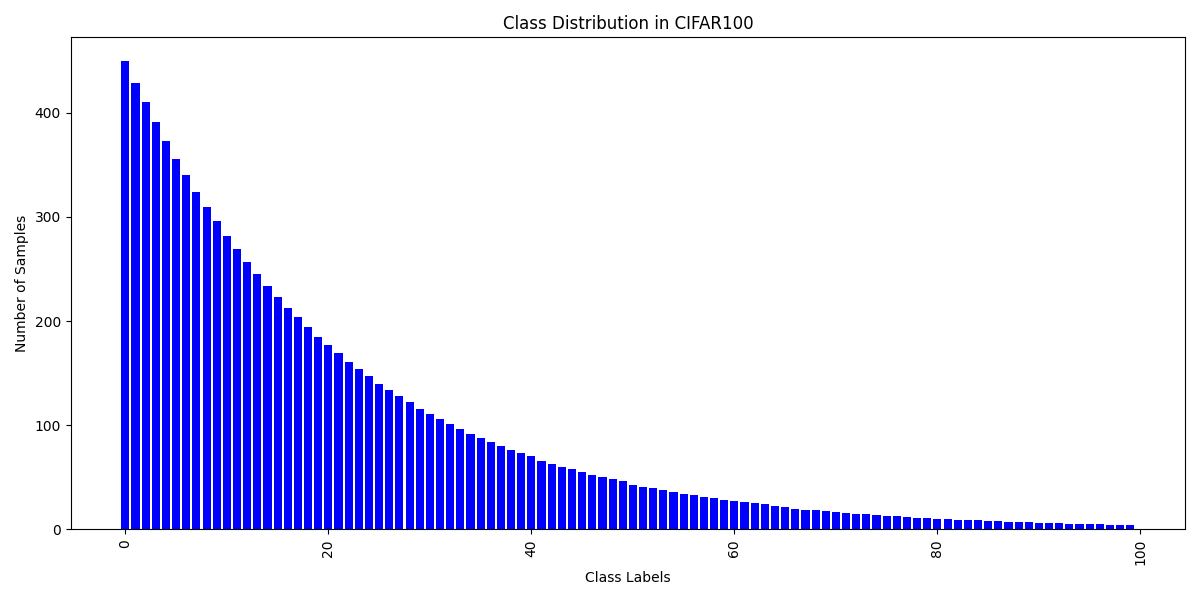
\includegraphics[width=0.9\textwidth]{Images/Plots/cifar100_train_450_imb.png}
    \caption{The class distribution of the CIFAR-100 long-tailed training set with 450 samples in the most frequent class.}
    \label{fig:cifar100_train_450_imb}
\end{figure}

\textbf{Test Set:} To evaluate the performance of the model under similar conditions to the imbalanced training set, an imbalanced test set was created from the previously split test dataset. The imbalance in the test set mirrors the exponential distribution used for the training data, with the same imbalance factor of 0.01. The class distribution in the test set follows the same order of classes (from most to least frequent) as the imbalanced training set. No class has fewer than one sample. The class distribution can be seen in figure \ref{fig:cifar100_test_imb}.

% \begin{figure}[h!]
%     \centering
%     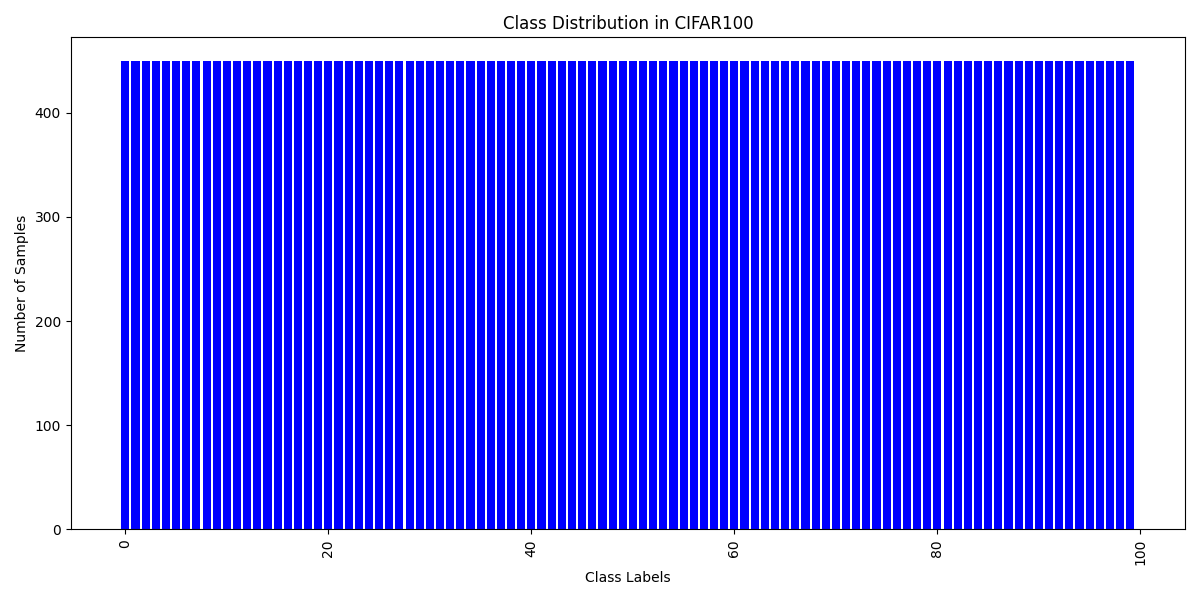
\includegraphics[width=0.9\textwidth]{Images/Plots/cifar100_bal_train_450.png}
%     \caption{The class distribution of the CIFAR-100 balanced training set with 450 samples per class.}
%     \label{fig:cifar100_train_450}
% \end{figure}



\begin{figure}[h!]
    \centering
    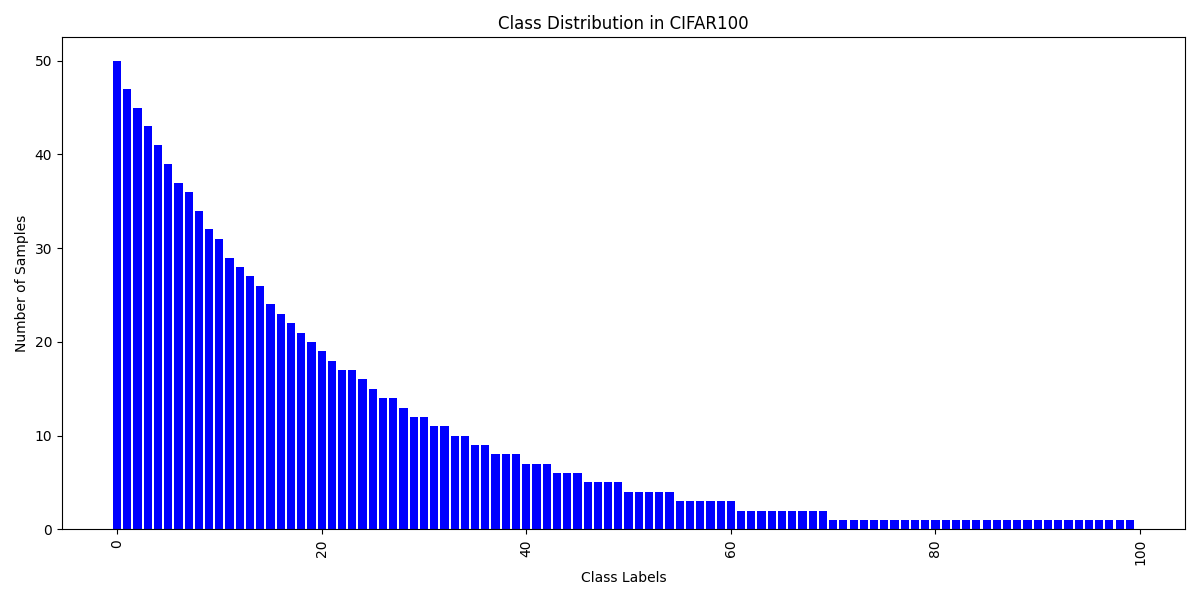
\includegraphics[width=0.9\textwidth]{Images/Plots/cifar100_test_imb.png}
    \caption{The class distribution of the CIFAR-100 long-tailed test set with 50 samples in the most frequent class.}
    \label{fig:cifar100_test_imb}
\end{figure}

\begin{figure}[h!]
    \centering
    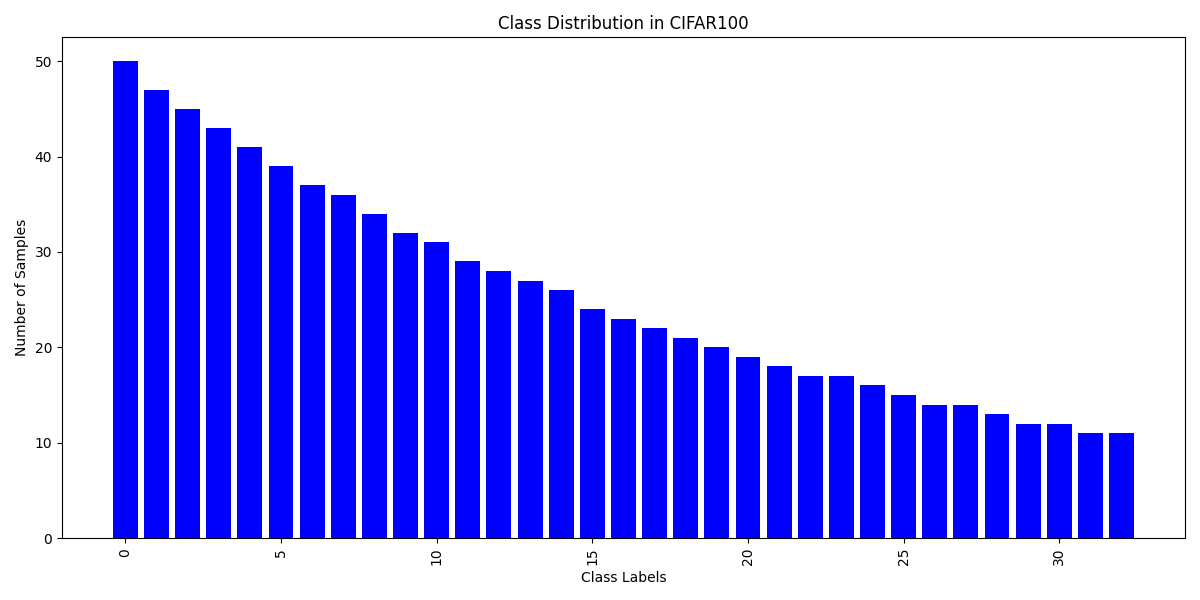
\includegraphics[width=0.9\textwidth]{Images/Plots/cifar100_test_head.png}
    \caption{The class distribution of the CIFAR-100 long-tailed test head classes.}
    \label{fig:cifar100_test_head}
\end{figure}


\begin{figure}[h!]
    \centering
    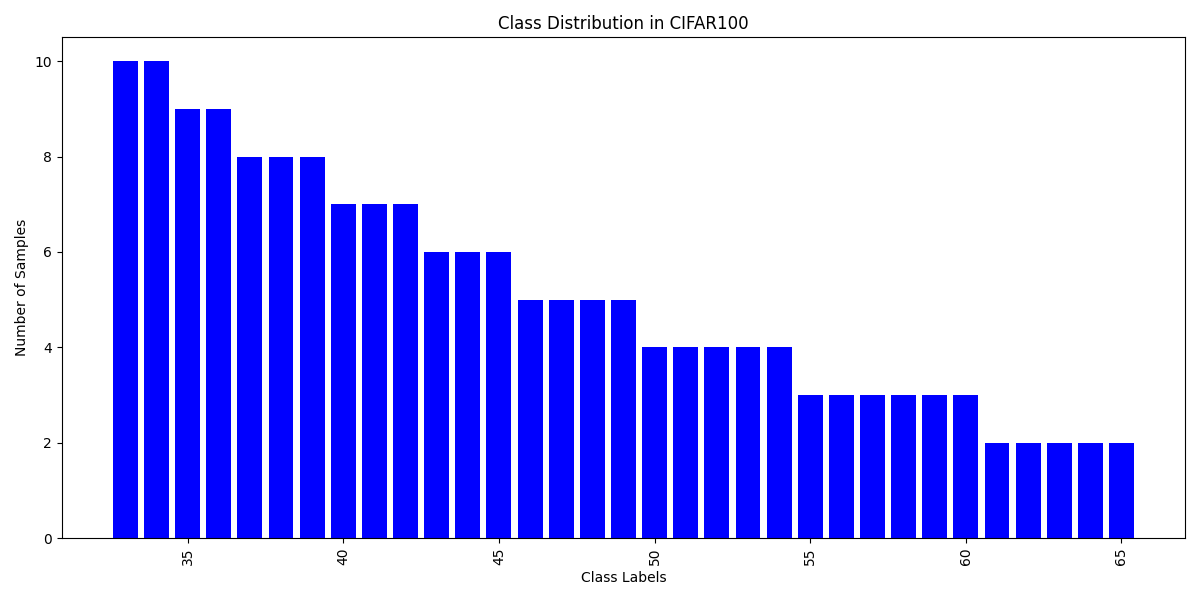
\includegraphics[width=0.9\textwidth]{Images/Plots/cifar100_test_middle.png}
    \caption{The class distribution of the CIFAR-100 long-tailed test middle classes.}
    \label{fig:cifar100_test_middle}
\end{figure}

\begin{figure}[h!]
    \centering
    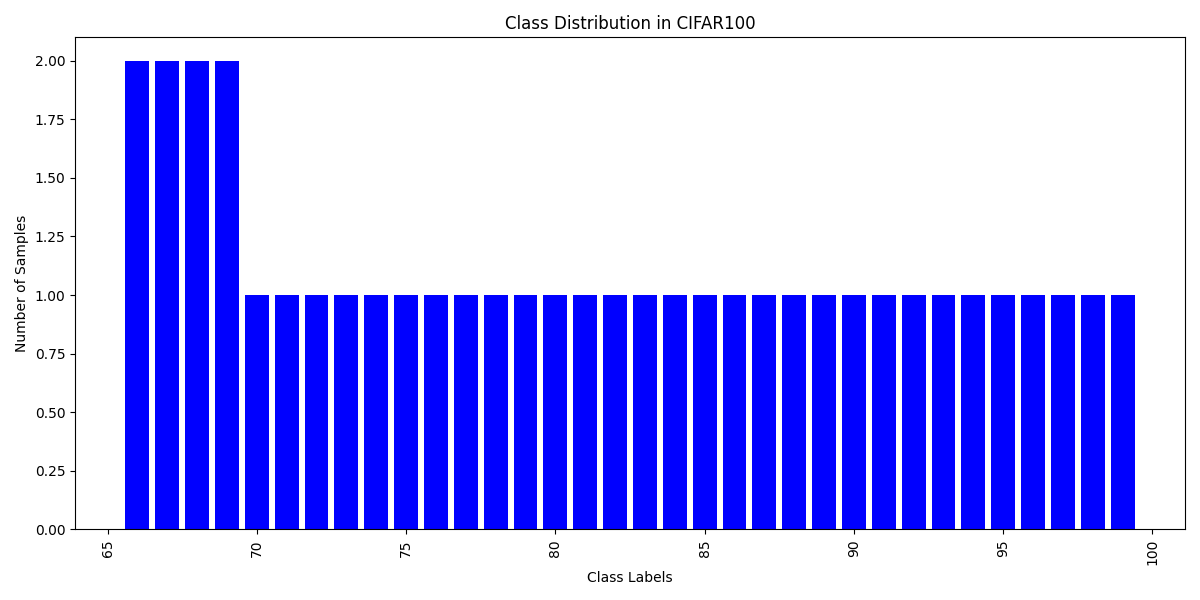
\includegraphics[width=0.9\textwidth]{Images/Plots/cifar100_test_tail.png}
    \caption{The class distribution of the CIFAR-100 long-tailed test tail classes.}
    \label{fig:cifar100_test_tail}
\end{figure}


\subsection{Data Augmentation}
Data augmentation and normalization were applied to the CIFAR-100 dataset to improve model generalization and align the preprocessing with the dataset's characteristics. While the models used in this study were pretrained on ImageNet, the normalization process was based on the CIFAR-100-specific RGB statistics: mean values of [0.4914, 0.4822, 0.4465] and standard deviations of [0.2023, 0.1994, 0.2010]. This decision was made to tailor the preprocessing to the pixel value distribution of CIFAR-100, ensuring that the input normalization better reflected the properties of the dataset used for fine-tuning and evaluation.

Although ImageNet statistics are often used with pretrained models to maintain consistency with the original training setup, they represent a different pixel value distribution. CIFAR-100, being a smaller dataset with distinct image characteristics, benefits from normalization based on its own statistics. This approach reduces the domain gap between the preprocessing and the dataset, potentially allowing the models to learn more effectively from the CIFAR-100-specific data distribution.

By using CIFAR-100 statistics, this study aims to strike a balance between leveraging the advantages of ImageNet pretraining and adapting the models to the unique properties of the target dataset. Future work could explore the impact of using ImageNet statistics instead to assess the trade-offs between these two approaches.

\section{Long-tailed Learning Techniques}
Description of the specific methods used to address class imbalance, such as data sampling, class re-weighting, etc. 
Justification for selecting these techniques, potentially referencing prior research (from Deep Long-Tailed Learning: A Survey by Zhang et al.).

\subsection{Model Selection}
\textit{A list of subjects to include in this section:}

\begin{itemize}
    \item Mention the model architectures chosen for training, and describe why they are appropriate for deep long-tailed learning with reference to the background section.
    \item Discuss the strengths and limitations of these models in addressing the challenges posed by imbalanced data.
    \item Describe how they were pretrained (ImageNet-1K, ImageNet-21K) and what that means for the training on CIFAR100.
\end{itemize}


\subsection{Selection of Loss Function}
\textit{A list of subjects to include in this section:}

 \begin{itemize}
    \item Describe the different loss functions and why they are appropriate for deep long-tailed learning with reference to the background section.
    \item Rationale for each loss function's inclusion, focusing on its expected benefits for imbalanced classes and how it adresses the bias toward majority classes.
    \item Write pseudo code of the implementations
 \end{itemize}

 \paragraph{Softmax Loss}
 Without any additional weighting or margin adjustments, the standard CE loss tends to give well-represented classes an advantage. Since head classes have more training examples, each of their samples also serves as a “negative” example for all other classes, providing them with a disproportionately high number of beneficial gradients. In contrast, tail classes, having fewer positive samples, are both less represented positively and more often negatively suppressed \cite{zhang2023deep, lin2018focallossdenseobject}. As a result, the model learns biased decision boundaries, performing well on frequent classes but poorly on rare ones. The CE loss thus serves as a natural starting point or baseline from which various class-sensitive modifications are derived. These modifications directly address the imbalance issue by altering the training dynamics, ensuring a more equitable distribution of gradients and improving the final model’s performance on underrepresented classes.

 \paragraph{Weighted Softmax Loss}
 (1) In scenarios of severe imbalance, minority classes are often overshadowed by the abundant head classes. WCE addresses this by scaling the loss for each class according to a class-dependent factor, typically the inverse of its frequency, thereby placing a heavier penalty on misclassification of rare classes \cite{zhang2023deep}.
(2) By elevating the importance of tail classes in the loss, the model is incentivized to allocate more representational capacity to them, improving recall and reducing class-specific error rates.
(3) Although simple, WCE provides a direct and intuitive method for re-weighting: each class’s contribution to the parameter updates is modulated to reflect its scarcity or importance in the dataset distribution.
(4) This helps maintain a more balanced gradient flow during training, preventing head classes from monopolizing the optimization trajectory.
(5) However, one limitation is that the choice of class weights is often empirical. Naively using the inverse class frequency may not always yield optimal results, and more sophisticated weighting heuristics or data-driven methods can be employed \cite{zhang2023deep}.
(6) WCE sets a straightforward precedent for other re-weighting schemes, serving as a baseline for more elaborate methods that try to adapt the weights dynamically during training.
(7) As it is easy to implement and understand, WCE is frequently considered as an initial step towards handling imbalance before exploring more complex techniques.
(8) Overall, WCE exemplifies how re-weighting can effectively guide the model to learn less-represented categories more robustly, thereby improving long-tailed recognition performance.

\paragraph{Focal Loss}
(1) Focal Loss modifies the CE loss by including a focusing parameter that down-weights well-classified examples, thus reducing the dominance of easily recognized classes or samples \cite{lin2018focallossdenseobject}.
(2) By concentrating on hard examples—often those from underrepresented classes—Focal Loss ensures that the model’s parameter updates focus on improving performance where it struggles the most.
(3) This dynamic weighting effectively reduces the overwhelming influence of head classes, since these classes tend to produce more confidently correct predictions that are down-weighted.
(4) Consequently, tail classes, which inherently present more challenging classification problems, receive increased attention and a larger share of meaningful updates.
(5) The intuition is that by penalizing confident yet trivial predictions less, the model has “budget” to allocate its learning capacity towards harder or rarer samples, thereby mitigating the imbalance effect.
(6) Empirical results have shown that this approach can significantly boost performance on minority classes without severely degrading performance on majority classes \cite{zhang2023deep}.
(7) Since Focal Loss does not depend solely on class frequency, it can adapt to the evolving difficulty distribution of samples during training, making it more flexible than static frequency-based weights.
(8) Though originally introduced in the context of object detection, it has been widely adopted in image classification tasks with long-tailed distributions.
(9) Thus, Focal Loss stands as a prime example of a re-weighting strategy that leverages model feedback (prediction confidence) rather than static priors (class frequencies) to balance training.

\paragraph{Class-Balanced Loss}
(1) The key insight is that each class’s influence should not be linearly scaled by its frequency alone. Instead, it considers that as class size grows, its incremental value decreases, suggesting that fewer samples are needed from frequently seen classes to establish robust representations.
(2) By formulating a class-specific weight derived from the effective sample number, CB Loss prevents large classes from dominating the training gradient simply due to their sheer volume of examples.
(3) This leads to a more stable and theoretically grounded re-weighting mechanism than naive inverses of class frequency, and can yield better generalization on minority classes.
(4) The concept of effective number is computed using a parameter $\gamma$ to determine how quickly the marginal benefit of additional samples decreases.
(5) This approach balances the training signal by giving classes a weight proportional to the inverse of their effective number, essentially normalizing the influence of different classes to a more comparable scale \cite{zhang2023deep}.
(6) As a result, CB Loss ensures that each class, regardless of its raw frequency, contributes meaningful gradients that reflect both its representation level and its effective complexity.
(7) This method elegantly merges the ideas of frequency-based weighting with a diminishing return model, acknowledging that overly abundant classes do not linearly improve overall performance.
(8) With this refined weighting scheme, CB Loss tends to improve recognition of rare categories without unduly harming head class accuracy.
(9) In effect, CB Loss provides a solid theoretical foundation for re-weighting by linking data volume, information content, and balanced training signals.

\paragraph{Balanced Softmax Loss}
(1) Standard softmax-based training assumes a balanced class distribution during both training and testing, which is often unrealistic in real-world datasets.
(2) BS Loss recognizes that applying a correction to the logits rather than just weighting the final loss terms can more directly counter the skewed gradient flow that results from class imbalance \cite{zhang2023deep}.
(3) By multiplying logits by the class frequencies, it effectively adjusts the decision boundaries, ensuring that classes with fewer samples are not overshadowed by the dense representation of majority classes.
(4) This adjustment encourages the model to produce a more uniform posterior distribution that accurately reflects true class priors, both during training and inference.
(5) Consequently, the network learns a more balanced internal representation, fostering improved recognition of tail classes without overly penalizing head classes.
(6) Balanced Softmax offers a theoretically motivated way to incorporate known label distributions into the training process, aiming to produce unbiased probability estimates.
(7) It can be seen as a more direct approach to re-weighting at the logit level, contrasting with methods that focus on re-weighting the loss function after probability computation.
(8) Empirical results show that BS Loss can be more effective than naive weighting schemes, as it corrects the bias at its source rather than compensating after the fact.
(9) This method paves the way for other logit-adjustment techniques and underscores the importance of integrating class priors into the model’s probability estimation process.

\paragraph{Equalization Loss}
(1) In highly imbalanced scenarios, each positive sample from a head class can produce negative gradients for all other classes, including tail classes. Over time, this can discourage the network from correctly identifying these minority classes.
(2) EQ Loss counteracts this by selectively down-weighting the negative gradients that arise when tail classes appear as negative samples for majority classes \cite{zhang2023deep}.
(3) By reducing the negative influence on tail classes, EQ Loss ensures that the model does not develop an overly “head-biased” representation that fails to recognize minority categories.
(4) This strategy highlights a subtlety in the re-weighting paradigm: it is not only about boosting tail class importance, but also about preventing undue suppression of these classes through negative gradients.
(5) However, excessively down-weighting negative gradients may impair the model’s discriminative power. To address this, adaptive variants, such as ACSL and Equalization v2, adjust the amount of gradient suppression based on the model’s prediction confidence \cite{tan2020equalizationlosslongtailedobject, zhang2023deep}.
(6) This adaptive mechanism allows the network to selectively protect tail classes when needed, while still maintaining a strong discriminative boundary between classes.
(7) The result is a more balanced training signal that prevents rare classes from being “washed out,” thereby improving long-tailed recognition.
(8) EQ Loss exemplifies a more fine-grained approach to re-weighting, intervening at the gradient level to ensure fair treatment of minority categories.
(9) By focusing on the gradient flow rather than just the static weighting of loss values, EQ Loss and its successors illustrate the evolving sophistication of class-sensitive re-weighting techniques.

\paragraph{LDAM Loss}
(1) Margin-based losses generally improve generalization by enforcing a minimum separation between class decision boundaries.
(2) LDAM incorporates class-dependent margins that are inversely related to class frequencies, providing larger margins to tail classes and smaller margins to head classes \cite{zhang2023deep}.
(3) By increasing the margin for minority classes, it effectively lowers their decision boundary threshold, making it easier for the model to confidently classify these classes and reducing their misclassification rates.
(4) This approach contrasts with re-weighting methods: while re-weighting modifies the magnitude of the loss contributions, re-margining directly influences how decision boundaries are formed in the embedding space.
(5) The motivation behind LDAM is that the imbalance problem is not solely a matter of loss amplitude, but also how easily minority classes can carve out their own regions in the feature space.
(6) With larger margins for tail classes, LDAM encourages more robust and discrimination-friendly representations for these classes, thereby counteracting the bias induced by uneven sample distributions.
(7) As a result, the final classifier tends to perform better on rare categories, as it learns to keep them well-separated from other classes, even when their sample counts are low.
(8) Combining LDAM with re-weighting or re-sampling techniques can yield even stronger improvements, as each method addresses a complementary aspect of the imbalance issue.
(9) LDAM underscores that balancing the training process can be achieved not only by adjusting loss weights, but also by reshaping the geometry of the decision boundaries in class-sensitive ways.

\subsection{Excluded Long-Tailed Learning Methods}
This section will explain why some deep long-tailed learning techniques, like re-sampling, was not the focus of this thesis.

\section{Evaluation Metrics}
\textit{A list of subjects to include in this section:}

\begin{itemize}
    \item Describe common evaluation metrics used for classification tasks.
    \item Explain the choice of top-1 accuracy.
    \item Explain how the performance is assessed across different class groups.
    \item Explain the choice of F1-score.
\end{itemize}



\subsection{Model Comparison}
Metrics for comparison of overall model performance. Example: harmonic mean, geometric mean, min score. Mention why these metrics are suitable for balancing performance across head, middle, and tail classes.

\section{Reproducibility}
\textit{A list of subjects to include in this section:}

\begin{itemize}
    \item Use of random seed initialization.
    \item Documentation of dataset versions and codebase.
    \item Availability of scripts for dataset preparation and model training.
\end{itemize}

\section{Implementation Details}
Technical explanations of any unique or customized methods implemented in code, for example the custom dataset.

\textit{A list of subjects to include in this section:}

\begin{itemize}
    \item Explain how the models where implemented.
    \item Rationale for implementing the loss functions manually instead of copy existing repositories.
    \item Describe the benefits of copying existing repositories.
\end{itemize}

